\hypertarget{architecture__concepts_fundamental_structure}{}\subsection{Fundamental Structure}\label{architecture__concepts_fundamental_structure}



\begin{DoxyImage}
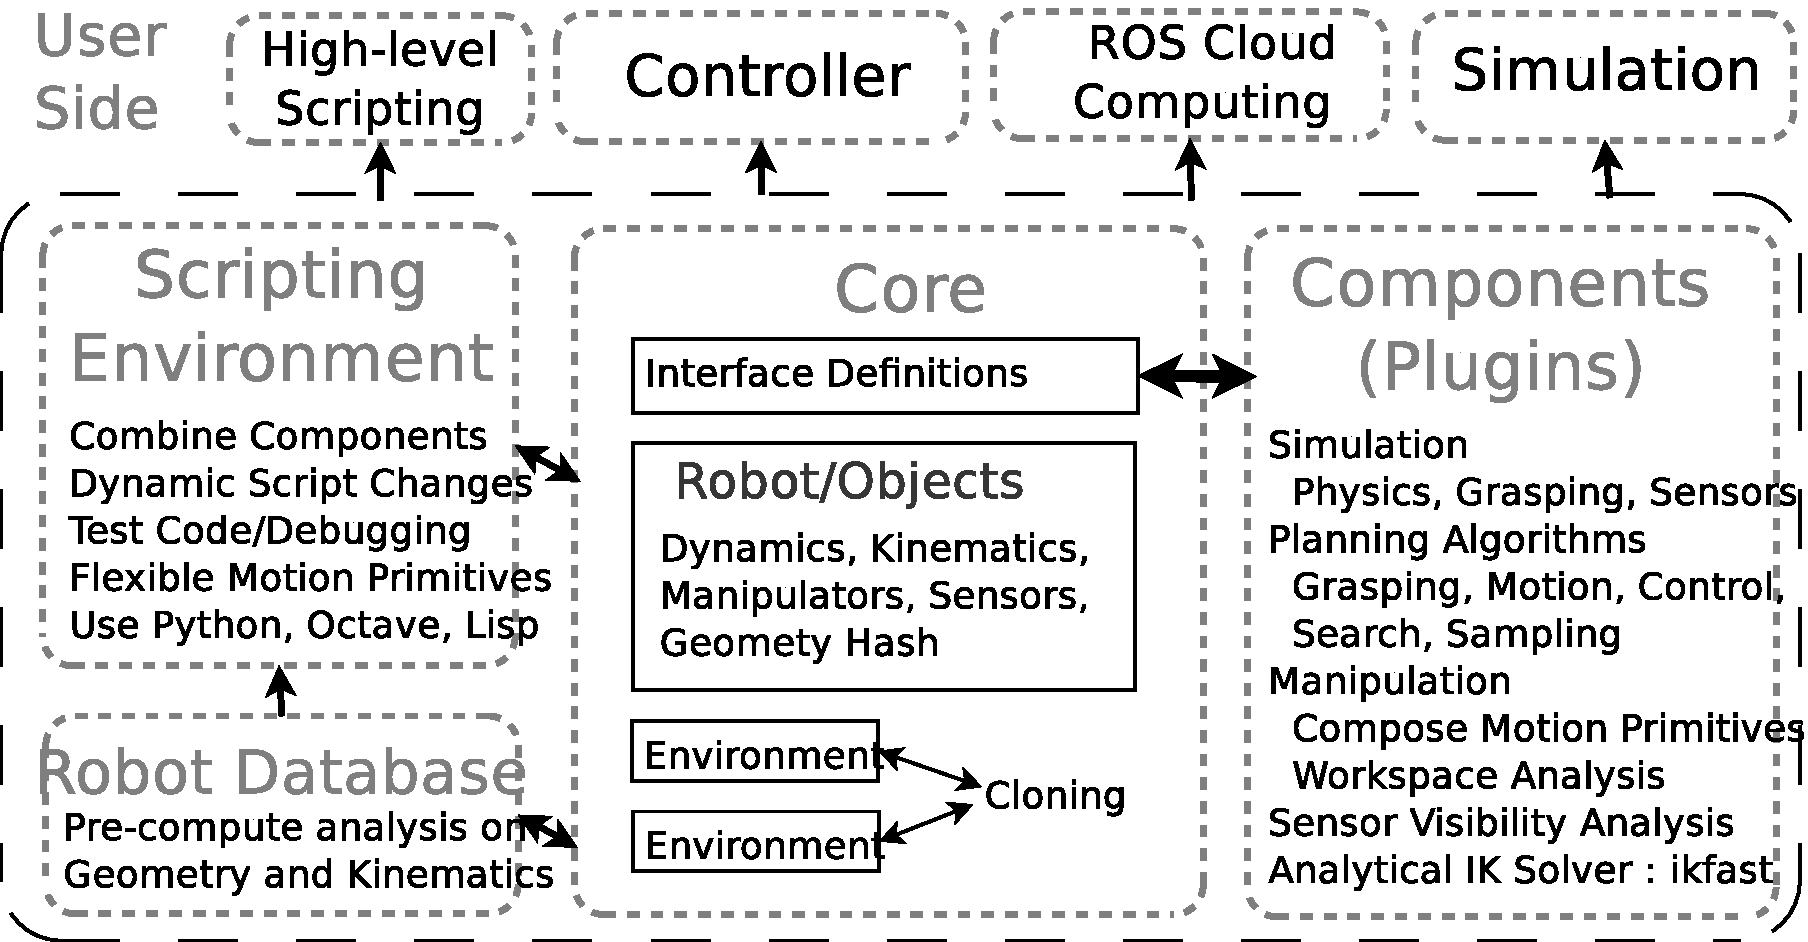
\includegraphics[width=15cm]{openrave_architecture}
\caption{OpenRAVE architecture}
\end{DoxyImage}


OpenRAVE is divided in four main components as shown in the above figure:


\begin{DoxyItemize}
\item {\bfseries Core Layer} The core is composed of a set of \hyperlink{group__interfaces}{Base Interface Classes} defining how plugins share information, and it provides an environment interface that maintains a world state, which serves as the gateway to all functions offered through OpenRAVE. The global openrave state manages the loaded plugins, multiple independent environments, and logging. On the other hand, the \hyperlink{classOpenRAVE_1_1EnvironmentBase}{environment} combines collision checkers, viewers, physics engines, the kinematic world, and all its interfaces into a coherent robotics world state.
\end{DoxyItemize}


\begin{DoxyItemize}
\item {\bfseries Plugins Layer} OpenRAVE is designed as a plugin-\/based architecture where a plugin offers implementations of the \hyperlink{group__interfaces}{Base Interface Classes} that are loaded dynamically into the \hyperlink{classOpenRAVE_1_1EnvironmentBase}{environment}. Plugins can be linked with other robotics libraries allowing \hyperlink{namespaceOpenRAVE}{OpenRAVE} to expand its functionality, or it can offer \hyperlink{namespaceOpenRAVE}{OpenRAVE} services to another robotics system. During startup, OpenRAVE parses the \{OPENRAVE\_\-PLUGINS\} environment variable and loads all the plugins it finds.
\begin{DoxyItemize}
\item Refer to \hyperlink{writing__plugins}{Writing Plugins and Interfaces} for a tutorial on how to build and compile plugins.
\item Refer to \hyperlink{interface__concepts}{Base Interface Concepts} for interface details.
\end{DoxyItemize}
\end{DoxyItemize}


\begin{DoxyItemize}
\item {\bfseries Scripting Layer} OpenRAVE provides scripting environments for \href{http://openrave.org/en/main/tutorials/openravepy_beginning.html#openravepy-beginning}{\tt Python} and \href{http://openrave.org/wiki/index.php/OctaveMATLAB}{\tt Octave/Matlab}. Python communicates with the core layer directly with in-\/memory calls, making it extremely fast. On the other hand, the Octave/Matlab scripting protocol send commands through TCP/IP, with a plugin offering a text server on the OpenRAVE core side. Scripting allows real-\/time modifications to any aspect of the environment without requiring shutdown, making it ideal to testing new algorithms. The Python scripting is so powerful, that most of the OpenRAVE examples and demo code are offered through it. In fact, users should treat the scripting language as an integral part of the entire system, not as a replacement to the C++ API.
\end{DoxyItemize}


\begin{DoxyItemize}
\item {\bfseries Robot Database Layer} Implements a planning knowledge-\/base and provides simple interfaces for its access and generation parameters. The database itself mostly consists of kinematic, quasi-\/static, dynamic, and geometric analyses of the robot and the task. If the robot is defined properly, then all these functions should work out of the box.
\end{DoxyItemize}

All the base planners and modules should be applicable to any robot structure that can be thrown at it. One of OpenRAVE's strongest points when compared with other planning packages is the idea of being able to apply algorithms in openrave to any robot, with very little modification. Recently, a planning database structure has been introduced that allows computation of properties like convex hull decomposition, grasp sets, reachability maps, analytic inverse kinematics, etc. If the robot is defined properly, then all these functions should work out of the box.

The main API is coded in C++ using the Boost C++ libraries \mbox{[}Dawes et al (1998-\/ present)\mbox{]} as a really solid basis of low-\/level management and storage structures. The Boost flavors of shared pointers allow object pointers to be safely reference counted in a heavily multi-\/threaded environment. Shared pointers also allow handles and interfaces to be passed to the user without having to every worry about the user calling upon invalid objects or un-\/ loaded shared objects. Furthermore, \hyperlink{namespaceOpenRAVE}{OpenRAVE} uses functors and other abstracted objects commonly seen in higher level languages to specify function pointers for sampling distri-\/ butions, event callbacks, setting robot configuration state, etc. The Boost-\/enabled design makes the the C++ API really safe and reliable to use along with saving the users a lot of trouble doing bookkeeping on their end. Furthermore, it allows the Resource Acquisition Is Initialization (RAII) design pattern \mbox{[}Stroustrup (2001)\mbox{]} to be fully exploited allowing users to ignore the complexities of multi-\/threaded resource management.\hypertarget{architecture__concepts_arch_environment}{}\subsection{Environment Concepts}\label{architecture__concepts_arch_environment}
All of OpenRAVE's services are offered through the environment. For example, requesting a planner interface called 'BiRRT' is done through RaveCreatePlanner(). The environment supports:


\begin{DoxyItemize}
\item \hyperlink{namespaceOpenRAVE_global_functionality}{managing and communicating with plugins}
\item \hyperlink{classOpenRAVE_1_1EnvironmentBase_env_collision_checking}{collision checking}
\item \hyperlink{classOpenRAVE_1_1EnvironmentBase_env_loading}{loading scenes and objects}
\item \hyperlink{classOpenRAVE_1_1EnvironmentBase_env_objects}{managing objects and triangulation}
\item \hyperlink{classOpenRAVE_1_1EnvironmentBase_env_plotting}{drawing/plotting}
\end{DoxyItemize}

Whenever objects in the environment are written or read, the user has to {\bfseries lock} the environment mutex mutex GetMutex(). This prevents any other process from modifying the enviornment while the user is working. Because the environment uses 'recursive mutexes, it allows a mutex to be locked as many times as needed within the same thread. This has allowed all environment functions that require locking to always guarantee the mutex is locked, regardless if the user has locked the mutex. (Note that this only applies to environment functions, and not interface functions).\hypertarget{architecture__concepts_arch_locking}{}\subsubsection{Locking}\label{architecture__concepts_arch_locking}
Because OpenRAVE is a highly multi-\/threaded environment, the environment state like bodies and loaded interfaces could be simultaneously accessed. In order to safely write or read the state, a user has to lock the environment, which prevents any other process from modifying the environment while the user is working. By using recursive locks, it allows a lock to be locked as many times as needed within the same thread, greatly reducing the lock management when a state changing function calls another state changing function. This safety measure helps users by always guaranteeing the environment is locked when calling global level environment functions like creating new bodies or loading scenes, regardless if the user has locked it. However, directly accessing the bodies and robots is dangerous without having the environment lock acquired.\hypertarget{architecture__concepts_arch_simulation}{}\subsubsection{Simulation Thread}\label{architecture__concepts_arch_simulation}
Every environment has an internal time and a simulation thread directly attached to a physics engine. The thread is always running in the background and periodically steps the simulation time by a small delta for the physics engine and on all the simulation-\/enabled interfaces. By default, the thread is always running and can always potentially modify the environment state; therefore, users always need to explicitly lock the environment whenever playing with the internal state like modifying bodies by setting joint values or link transformations. If not careful, the controller or physics engine will overwrite them. By default, the simulation thread just sets the object positions depending on their controller inputs, but a physics engine can be attached to integrate velocities, accelerations, forces, and torques.

The simulation thread can feel like a nuisance at first, but its division of robot control into control input computation and execution greatly helps users only concentrate on feeding commands to the robot without worrying about the simulation loop. It also allows a world update to happen in one one discrete time step.\hypertarget{architecture__concepts_arch_cloning}{}\subsubsection{Cloning}\label{architecture__concepts_arch_cloning}
One of the strengths of OpenRAVE is in allowing multiple \hyperlink{classOpenRAVE_1_1EnvironmentBase}{environments} work simultaneously in the same process. Environment cloning allows OpenRAVE to become truly parallel by managing multiple environments and running simultaneous planners on top of them.

One of the strengths of \hyperlink{namespaceOpenRAVE}{OpenRAVE} is in allowing multiple environments to work simul-\/ taneously in the same process. Environment cloning allows \hyperlink{namespaceOpenRAVE}{OpenRAVE} to become truly parallel by managing multiple environments and running simultaneous planners on top of them. Because there is no shared state across the clone and the original environment, it is not possible to use an interface created from one environment in another For example, if a planner is created in one environment, it should be used only by objects in that environment. It is not possible to set a planner to plan for objects belonging to a different environment. This is because a planner will lock the environment and expect the objects it controls to be exclusively under its control.

Creating a clone is simple, in C++ just type:


\begin{DoxyCode}
EnvironmentBasePtr pNewEnvironment = GetEnv()->CloneSelf(Clone_Bodies)
\end{DoxyCode}


to create a clone that copies all the existing bodies (with attachments and grabbed bodies) and their current states. Basically the clone can perform any operations that would have been done with the original enviornment.

Because the environment state is very complex, the cloning process can control how much of it gets transferred to the new clone. For example, all existing bodies and robots can be cloned, their attached controllers can be cloned, the attached viewer can be cloned, the collision checker state can be cloned, and the simulation state can be cloned. Basically the clone should be able to perform any operations that can be done with the original environment without any modification in the input parameters.

When cloning real robots, one extremely important feature that \hyperlink{namespaceOpenRAVE}{OpenRAVE} cloning offers is the ability to maintain a real-\/time view of the world that sensors continuously update with new information. When a planner is instantiated, it should make a copy of the environment that it can exclusively control without interfering with the updating operations. Furthermore, the real-\/world environment possibly has robot controllers connected to real robots, having a clone gives the ability to set simulation controllers guarantees robot safety while planning; commands from a cloned environment would not accidentally send commands to the real robot.\hypertarget{architecture__concepts_arch_validating_plugins}{}\subsubsection{Validating Plugins}\label{architecture__concepts_arch_validating_plugins}
Every plugin needs to export several functions to notify the core what interfaces it has and to instantiate the interfaces. When a plugin is first loaded, it is validated by the environment and its interface information is queried so the core can register the names.

There are many mechanisms in the validation process to prevent old plugins to be loaded by the core. \hyperlink{namespaceOpenRAVE}{OpenRAVE} is updated frequently and all user plugins are not necessarily recompiled when the \hyperlink{namespaceOpenRAVE}{OpenRAVE} API changes. Therefore, we will encounter many cases when a plugin exports the correct functions, but does not implement the correct API. Using interfaces from plugins compiled with a mismatching The API can lead to unexpected crashes that are very difficult to debug, so it is absolutely necessary to detect this condition. One possible solution is to add version numbers to the API to enforce checking before an interface is returned from the plugin to the environment, but this method is brittle. It forces to keep track of a version number for every interface along with a global version number. Furthermore, every developer has to remember to increment the version when something even small changes, which can be easily forgotten and lead to serious errors later on.

We solve interface validation by computing a unique hash of the interface functions and members by running each interface through a C++ lexer, gathering the tokens that affect the C++ code structure, and then creating a 128bit unique MD5 hash. We create a hash for each interface definition and the environment. The hashes are hard coded into the C++ header files and can be queried by two methods: a static function returning the hash of the program calling the function, and a virtual function returning the hash the interface was compiled with. An interface is only valid if its virtual hash is equivalent to the static hash of the core environment. For a plugin to be loaded correctly, first the environment hashes have to match. If they do, then the individual interfaces checked and only matching interfaces are returned to the core, and from there dispatched to other plugins. Such consistency checks ensure that stale plugins will never be loaded.\hypertarget{architecture__concepts_arch_cloning_parallel}{}\subsubsection{Parallel Execution}\label{architecture__concepts_arch_cloning_parallel}
Being able to execute a planner in multiple threads is important for applications that require speed and solution quality Because there is always a trade-\/off between solution quality and time of computation, some applications like industrial robots require the quickest and smoothest past to their destinations. Fortunately, environment cloning allows planners to create an independent environment for every thread they create, which enables them to call kinematics and collision functions in each respective thread without worrying about data corruption. Growing an RRT tree in a multi-\/threaded environment just requires one copy of the kd-\/tree structure to be maintained. The query operations mostly work with Euclidean distance on the configuration space, so are really fast. Furthermore, adding a new point takes O(log) time, so it shouldn’t be a bottleneck in the search process compared to collision checking. Finally, environment locking allows threads to gain exclusive access to the environment. The rule of thumb is that any interface belonging or added to the environment requires an environment lock before any of its methods can be called.\hypertarget{architecture__concepts_arch_dualnature}{}\subsection{Dual Simulation/Control Nature}\label{architecture__concepts_arch_dualnature}
\hyperlink{namespaceOpenRAVE}{OpenRAVE} can be simultaneously used as a simulation, a controller, or both at the same time. Here are a couple of things to keep in mind:


\begin{DoxyItemize}
\item It can be used as a simulator by attaching a physics engine and setting torques to the joints and applying forces to the links.
\end{DoxyItemize}


\begin{DoxyItemize}
\item The physics engine directly reflects the internal openrave state.
\end{DoxyItemize}


\begin{DoxyItemize}
\item A controller can be set that sets torques/velocities/positions to the physics engine every time step. Physics simulation time steps are constantly called in an internal \char`\"{}openrave thread\char`\"{} if simulations are set to true (default)
\end{DoxyItemize}


\begin{DoxyItemize}
\item The default physics engine doesn't touch the openrave state, nor does it simulate velocities or dynamics
\end{DoxyItemize}


\begin{DoxyItemize}
\item The default controller just sets positions at the specified times
\end{DoxyItemize}

This is why users need to explicitly lock the environment mutex whenever playing with the internal openrave state like setting joint values or link transformations (in planners for example). Otherwise, the controller or physics engine will overwrite them.\hypertarget{architecture__concepts_arch_exceptions}{}\subsection{Exception Handling}\label{architecture__concepts_arch_exceptions}
By using the C++ Standard and Boost libraries, \hyperlink{namespaceOpenRAVE}{OpenRAVE} can recover from almost all errors that a user can experience without causing the program to shutdown on the spot. Invalid pointer and out-\/of-\/range accesses are extremely dangerous because they can modify unrelated memory, which causes the program to crash at a place completely unrelated to the root cause of the problem. Avoiding such problems has been one of the the highest priorities for the design. The core always surrounds any user code coming from plugins and callbacks with try/catch blocks, this allows the core to properly handle the error and notify the user of a problem without tearing down the environment. Because exception handling is slow, there is a fine balance of when a function should return an error code and what it should throw an exception. In \hyperlink{namespaceOpenRAVE}{OpenRAVE}, exceptions should never occur in normal operation of the program, they should only be for unexpected events of the program. For example, planners failing is an expected event dependent on the current environment, so planners should return an error code with the cause of the failure rather than throw an exception. In other words, exceptions convey the structural errors of the program that point to places in the code that should be fixed by the user. The following operations should throw exceptions in \hyperlink{namespaceOpenRAVE}{OpenRAVE}:


\begin{DoxyItemize}
\item invalid plugin or interface hashes,
\item invalid commands being sent to interfaces,
\item invalid arguments passed to functions,
\item invalid pointers or out-\/of-\/range parts of lists are accessed,
\item environment is not locked when it should be
\item a resource is present when it should be,
\item a math operation is not consistent with the rest of the environment,
\item environment naming constraints are not maintained,
\item unrecognized enumerated types are given, and
\item instantiation order is not maintained.
\end{DoxyItemize}

Any type of boost error, or null pointer access throws an openrave\_\-exception. This greatly reduces the amount of error checking code people do. For example, C code usually has this pattern:


\begin{DoxyCode}
bool somefun(KinBodyPtr pbody)
{
    if( !pbody )
        return false;
    pbody->GetTransform();
    ...
}
\end{DoxyCode}


or


\begin{DoxyCode}
bool somefun(KinBodyPtr pbody)
{
    assert( !!pbody );
    pbody->GetTransform();
    ...
}
\end{DoxyCode}


If these checks are not done, the code would segfault. However, these checks can really clutter the code. In openrave, it is safe to get away with:


\begin{DoxyCode}
bool somefun(KinBodyPtr pbody)
{
    pbody->GetTransform();
    ...
}
\end{DoxyCode}


then for handling errors (for example in the most top-\/level script), do


\begin{DoxyCode}
try {
    ...
    somefun(pbody)
    ...
}
catch(const openrave_exception& ex) {
    RAVELOG_WARN("exception caught: %s\n",ex.what());
    if( ex.GetCode() == ORE_EnvironmentNotLocked ) {
        RAVELOG_WARN("user forgot to lock environment!\n");
    }
    ...
}
\end{DoxyCode}


When using openravepy in python, such unhandled C++ errors throw a python exception, which can be safely caught and processed there.\hypertarget{architecture__concepts_arch_body_hashes}{}\subsection{Hashes for Body Structure}\label{architecture__concepts_arch_body_hashes}
A new concept that came out of \hyperlink{namespaceOpenRAVE}{OpenRAVE} is the idea of creating unique hashes of a body’s structure. Every body has an online state that includes:


\begin{DoxyItemize}
\item names of the body, its links, its joints,
\item link transformations, velocities, and accelerations in the world,
\item and attached bodies.
\end{DoxyItemize}

All other information is independent of the environment and can be categorized into the kinematics, geometry, and dynamics of the body. Furthermore, robots have categories for attached sensors and manipulators. The planning knowledge-\/base stores all cached information about a body and a robot, so it needs an consistent way of indexing this information. Indexing by robot names is not reliable because it is very difficult to remind a user to change the name every time the body structure is changed. Therefore, \hyperlink{namespaceOpenRAVE}{OpenRAVE} provides functionality to serialize the different categories of a body and create a 128-\/bit MD5 hash. Each of the models in the planning knowledge-\/base relies on different categories of the robot. For example:


\begin{DoxyItemize}
\item inverse kinematics generation only uses the kinematics of a sub-\/chain of the robot defined by the manipulator and the grasp coordinate system,
\item kinematic reachability cares about the robot geometry of the manipulator because it implicitly stores self-\/collision results,
\item inverse reachability further uses the links connecting the base robot link to the base manipulator link,
\item grasping cares about the geometry of the target body and the kinematics and geometry of the gripper,
\item convex decompositions only care about the link geometry, and
\item inverse dynamics cares only about the dynamics properties of each link and the kinematics.
\end{DoxyItemize}

There are several challenges to developing a consistent index across all operating systems and compilers since floating point errors could creep in when normalizing floating-\/point values. However, the idea of such an index could greatly help in developing a worldwide robot database that anyone can use.\hypertarget{architecture__concepts_supported_formats}{}\subsection{Resource File Formats}\label{architecture__concepts_supported_formats}
\hyperlink{namespaceOpenRAVE}{OpenRAVE} defines its own  format that allows instantiation of any \hyperlink{namespaceOpenRAVE}{OpenRAVE} interface and quick builing of robots and and kinematics structures. The rigid body geometries resources can be specified in virtually any 3D file format. For example:


\begin{DoxyItemize}
\item iv, vrml, wrl, stl, blend, 3ds, ase, obj, ply, dxf, lwo, lxo, ac, ms3d, x, mesh.xml, irrmesh, irr, nff, off, raw
\end{DoxyItemize}

These files can be used inside the $<$geom$>$ tags, or can be read directly into any of the environment ReadRobotX and ReadKinBodyX methods to create a single world body.

\hyperlink{namespaceOpenRAVE}{OpenRAVE} also supports the \href{http://www.collada.org}{\tt COLLADA} international standard on 3D geometry and modeling. COLLADA is augmented with these \href{http://openrave.programmingvision.com/wiki/index.php/Format:COLLADA}{\tt OpenRAVE robot-\/specific extensions}.

\href{../main/robots_overview.html#file-formats}{\tt More information here.} 